It is of primary interest to apply the \gls{qmla} algorithm to real-life, experimental systems. 
In this chapter we devise an \gls{es} to operate in conjunction with experimental data 
    in order to characterise an electron spin in an \gls{nv} centre in diamond.
In particular, we model, through Hamiltonian terms, interactions between the spin and 
    the spin bath in which it resides,
    so that \gls{qmla} is finding an effective model for the open system dynamics.
\par

Here we will first introduce a basic picture of \glspl{nvc}, 
    using basic but nonstandard nomenclature for simplicity;
    for thorough descriptions of the underlying physics, readers are referred to \cite{doherty2013nitrogen}.
We next discuss the target system with respect to its modelling, 
    determining the suitable terms which \emph{might} represent the \gls{nvc}'s interactions, 
    to inform the starting point for the \gls{qmla}.
Finally we describe the implementation of an \gls{es} for the examination of the \gls{nvc},
    and the results of the \gls{qmla} procedure. 

\section{\gls{nv}-centres}
\label{sec:nv_centres}

\gls{nv} centers are point defects in diamond, 
    occuring naturally \cite{davies1976optical} or synthetically \cite{meijer2005generation, edmonds2012production}.
A substitutional \gls{nitrogen} isotope is embedded in a lattice of carbon atoms in diamond, 
    adjacent to a lattice vacancy, 
    such that it is surrounded by three \glspl{carbon} \cite{lenef1996electronic}. 
Of the \gls{nitrogen} atom's five valence electrons, three bond with nearby \glspl{carbon};
    the remaining two unbonded electrons for a lone pair and can be thought of as a single spin-$\frac{1}{2}$ particle. 
The adjacent lattice vacancy has three unbonded electrons, 
    two of which bond together leaving a single unpaired electron.
The single electron in the lattice vacancy, together with the effective lone pair of the \gls{nitrogen}, 
    form a a system of two spin-$\frac{1}{2}$ particles.
Such systems have been thoroughly studied; 
    of particular interest are the resultant \emph{triplet} states, 
    i.e. the allowed permutations of the two particles with total quantum spin $S=1$, 
    with magnetic spin multiplicity allowing $m_s = {-1, 0, 1}$, 
    giving rise to three distinct energy levels for the system. 
\par 

A \emph{manifold} is a set of states differing only slightly, 
    for example states near the absolute ground state manifold might differ only in magnetic spin quantum number,
    and can be characterised as the ground state manifold. 
We consider two principle manifolds of the system:
    the ground state and excited manifolds, each consisting of 
    three states, corresponding to the allowed values for magnetic spin $m_s$, see \cref{fig:nv_centre_energy_levels}a. 
For brevity, we denote states with reference to their magnetic spin and manifold, 
    e.g. the state in the ground state manifold with $m_s=0$ is denoted $\ket{m_s=0}_g$. 
In the absence of a magnetic field, the states corresponding to $\ket{m_s=\pm1}$ are degenerate, 
    but in the presence of a magnetic field, $B$, they have distinct energy levels, 
    referred to as the Zeeman effect, \cref{fig:nv_centre_energy_levels}b. 
\par 

We designate the state $\ket{m_s=0}_g$ as the basis state $\ket{0}=\icol{1 \\ 0}$, 
    and $\ket{m_s=-1}_g$ as $\ket{1}=\icol{0 \\ 1}$, 
    such that we have defined a qubit and computational basis, \cref{fig:nv_centre_energy_levels}d.
By shining a laser of $532$nm (green) on the \gls{nvc}, it is excited to the excited manifold, 
    from which it decays back to the ground state manifold. 
Importantly, the process of this decay can be exploited for the preparation of the \gls{nvc} in 
    the computational basis state $\ket{0}$. 
That is, the dominant decay process from $\ket{m_s=0}_e$ is 
    spin-preserving, so it ends in $\ket{m_s=0}_g$. 
On the other hand, had the \gls{nvc} been in the $\ket{m_s=\pm1}_e$,
    the dominant decay process is through a shelving (singlet) state, 
    and does not preserve spin, such that it also decays to the $\ket{m_s=0}_g$.
Therefore, irrespective of the initial state, 
    by shining the green laser on the \gls{nvc}, 
    it is most likely that it has been prepared in $\ket{m_s=0}_g = \ket{0}$, 
    providing us a starting point from which to perform computation.
\par 

The difference in energy between $\ket{0}$ and $\ket{1}$ is addressible optically: 
    by shining a \gls{mw} pulse at the \gls{nvc}, we can oscillate the qubit between the two levels. 
Likewise, having initialised the state to $\ket{0}$, we can perform a $\nicefrac{\pi}{2}$ rotation 
    about the logical $z$-axis, by running the \gls{mw} laser for half the time, 
    resulting in the state $\ket{+}$. 
We can similarly devise \gls{mw} radiation to achieve quantum gates and operations on our \gls{nvc} qubit.
We depict these cycles in \cref{fig:nv_centre_energy_levels}c. 
\par

\begin{figure}
    \begin{center}
        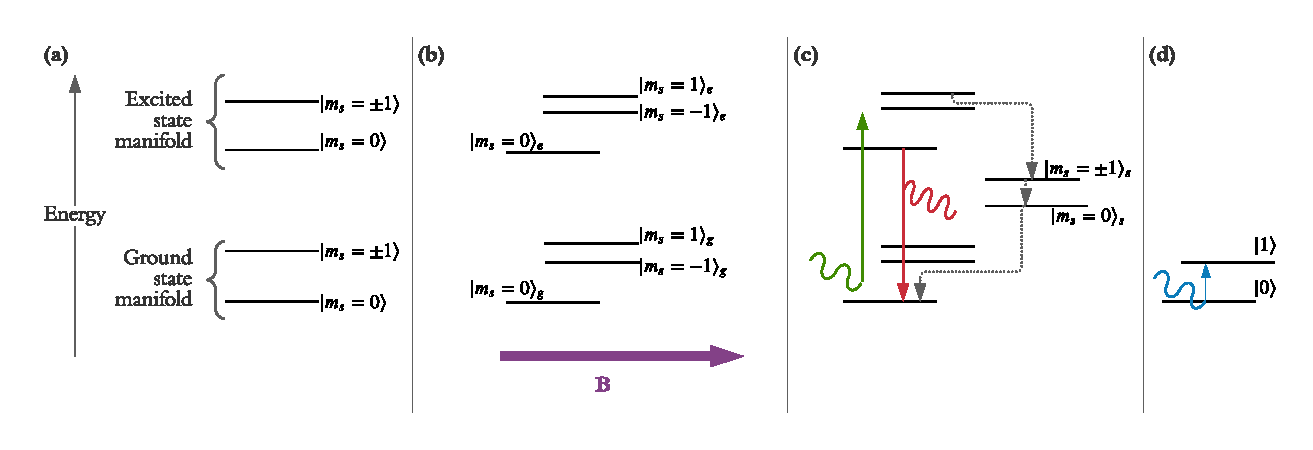
\includegraphics[width=0.8\linewidth]{experimental_study/figures/nv_centre_cartoon.pdf}
    \end{center}
    \caption[\glsentrylong{nvc} energy levels.]{
        Simplified depiction of energy levels of the \glsentrylong{nvc}, corresponding to its triplet state. 
        \textbf{a}, With no external field, the system simply has excited and ground-state manifolds, 
        each of which consist of two energy levels depending on the magnetic spin, $m_s$.
        \textbf{b}, In the presence of a magnetic field (purple, $B$), the magnetic spins have distinct energy levels, 
        i.e. Zeeman splitting. 
        States are denoted by their magnetic spin and subscripted by their manifold. 
        \textbf{c},  Application of a green ($532nm$) laser excites the \gls{nvc} from any of the states in the 
        ground state manifold to the excited manifold. 
        The dominant decay mechanism for the excited states are shown: 
            (i) $\ket{m_s=0}_e \rightarrow \ket{m_s=0}_g$ (red line) through the emission of a red ($637nm$) photon;
            (ii) $\ket{m_s=\pm 1}_e \rightarrow \ket{m_s=0}_g$ (dotted grey lines) via the shelving manifold which allows for non-spin-preserving transition, 
            and does not emit a photon. 
        \textbf{d}, Computational basis states $\ket{0}$ and $\ket{1}$ are assigned to the two lowest energy states.
            The difference in energy between these states is such that a microwave (MW, blue) photon
            can trigger transition from $\ket{0}$ to $\ket{1}$, as well as states in between such as $\ket{+}$, 
            allowing for the implementation of quantum logic gates. 
    }
    \label{fig:nv_centre_energy_levels}
\end{figure}


We can further exploit the decay mechanism to compose a readout procedure, 
    to infer the population of $\{\ket{0}, \ket{1}\}$ at a given instant, 
    for example following the application of gates to the system. 
We know that the excitation due to the green laser is spin-preserving, 
    i.e. when the \gls{nvc} has been excited to $\ket{m_s=0}_e$, 
    it had originated in $\ket{m_s=0}_g$.
We also know that the decay $\ket{m_s=0}_e \rightarrow \ket{m_s=0}_g$ is spin preserving, with the emission of 
    a red photon: by simply counting the number of photons emitted, we quantify the population of $\ket{0}$
    at the time of query. 
On the contrary, when the $\ket{m_s=-1}_g$ is excited, spin is also preserved, 
    so it goes to $\ket{m_s=-1}_e$;
    but $\ket{m_s=-1}_e$ decays 
    through the shelving state as outlined earlier, 
    \emph{without} the emission of a photon. 
We can hence infer the population of $\ket{m_s=-1}_g$ at the time of query by the fraction of incidents which don't emit a photon.
That is, say we first calibrate the system by retaining the green laser for some time: 
    after a few $\mu s$, a steady state is achieved where the majority of the time, the triplet is in the state $\ket{0} = \ket{m_s=0}_g$. 
Then, excitation from the same laser results in the excitation to $\ket{m_s=0}_e$, 
    which decays back to $\ket{m_s=0}_g$ and emits a photon in the process; 
    by counting the red photons emitted in a certain time window -- equivalently, measuring the \gls{pl} signal -- 
    we benchmark the population of $\ket{0}$ when nothing else has happened as $p_0$. 
Now, when we apply gates (i.e. \gls{mw} pulses) to the \gls{nvc}, 
    we can similarly read out the population of $\ket{0}$ as $p_0^{\prime}$,
    and infer that the likelihood that the \gls{mvc} is found in the initial state $\ket{0}$ is $\nicefrac{p_o^{\prime}}{p_0}$. 
We can use this quantity as the \gls{likelihood} within \gls{qle}, allowing us to learn from the \gls{nvc},
    as we will discuss in the next sections. 
\par 

In summary then, by assigning basis states $\ket{0}, \ket{1}$ to energy levels of the ground state manifold, 
    we are able to ensure the preparation of the \gls{nvc} in $\ket{0}$ by first shining a green laser on the \gls{nvc}. 
We can then apply \gls{mw} radiation to achieve quantum logical gates on the system, 
    and read out the final state of the system, again by shining a green laser
    and observing the emitted photons (\gls{pl}) and inferring the population level of each basis state. 
We represent these concepts in a simplified format in \cref{fig:nv_centre_energy_levels}. 


\section{Target system}
We take the axis of the \gls{nvc}, i.e. the axis connecting the \gls{nitrogen} with the 
    lattice vacancy, as the $z$-axis.
There are clearly a huge number of interactions to which the \gls{nvc} is subject:
    we choose to focus on its interactions with the environment, 
    i.e. with nuceli in the same diamond, which dictate its decoherence. 
These interactions are characterised by hyperfine terms \cite{smeltzer201113c}.
The overall Hamiltonian for such systems, where the set of nuclear sites is $\{\chi\}$,
    is given by 

\begin{equation}
    \label{eq:nv_ham_full}
    \hat{H}_{\mathrm{full}} 
    = 
    \Delta_{\textrm{gs}} \hat{S}_z^2 
    + \mu_B g \mathbf{B} \cdot \mathbf{S} 
    + \mathbf{S} \cdot \sum_{\chi} \left( \mathbf{A}_{\chi} \cdot \hat{I}_{\chi} \right) 
    + P \hat{I}_z^2 
    + \mu_n g \mathbf{B} \cdot \sum_{ \chi} \hat{I}_{\chi}.
\end{equation}

We will describe each term, as well as approximations which enable us to simplify the space considerably. 

\begin{easylist}[itemize]
    & Isolated-spin terms, i.e. describing the spin independent of the environmental nuclei
    && $\Delta_{\textrm{gs}} \hat{S}_z^2$: 
        the \emph{zero-field} splitting, 
        i.e. without any external (magnetic) field, the spin oscillates rapidly, with 
        $\Delta_{\textrm{gs}} \sim \tezxtrm{GHz}$. 
    && $\mu_B g \mathbf{B} \cdot \mathbf{S}$: 
        the spin's precession about the magnetic field, 
        $\mathbf{B} = \left(B_x \  B_y \  B_z\right)$, 
        via the total spin operator\footnotemark \ $\mathbf{S} = \left(\hat{S}_x \ \hat{S}_y \ \hat{S}_z \right)$, 
        where $\mu_B$ is the Bohr magneton and $g$ is the $g$-factor 
        ($\approx 2$, simplified from the g-factor tensor).
    
    & Hyperfine terms
    && $\hat{S} \cdot \sum_{\chi} \left( \mathbf{A}_{\chi} \cdot \hat{I}_{\chi} \right)$:
        The \gls{nvc} total spin operator $\mathbb{S}$ couples with each site, $\chi$.
        At each site there is a nucleus which has total spin operator 
        $\mathbf{I}_{\chi} = \left(\hat{I}_x \ \hat{I}_y \ \hat{I}_z \right)_{\chi}$. 
        $\mathbf{A}$ is the hyperfine tensor, containing the hyperfine parameters of interest. 

    & Bath-only terms, i.e. describing the other nuceli independent of the spin
    && $P \hat{I}_z^2 $: the quadrupole splitting, i.e. this term gives the splitting 
        of the \gls{nitrogen}'s hyperfine splitting, which does not meaningfully
        contribute to the short-decay processes in the experiments described in the next section. 
    && $\mu_n g \mathbf{B} \cdot \sum_{ \chi} \hat{I}_{\chi}$:
        $\mu_n$ is the nuclear magneton and $g$ is again the $g$-factor.
\end{easylist}

\footnotetext{
    We invoke an inexact representation of high dimensional tensors here for ease of interpretation. 
    For instance, the total nuclear spin operator exists in arbitrary dimension 
    (depending on the number of sites modelled), 
    but we present it simply as $\mathbf{I} = \left( \hat{I}_x \ \hat{I}_y  \ \hat{I}_z \right)$ at each site 
    to convey that we can separate the terms in the construction of models. 
}

Given that we are interested in the spin and its interactions with the environment only, 
    we can immediately drop the bath-only terms, by assuming the bath is static 
    apart from its interactions with the \gls{nvc}. 
This is a usual assumption in the treatment of open system dynamics, 
    to allow for focus on the dominant interactions for the system of interest \cite{breuer2002theory}. 
Additionally, since the zero field splitting contributes a constant shift in energy, 
    we can safely omit it by moving to the rotating frame. 
We are then left only with the second and third terms of \cref{eqn:nv_ham_full}. 

\subsection{Mapping to model terms}
Next we will focus on mapping the remaining terms to operators to compose the set of terms 
    $\termset$ to use in our \gls{es}. 
In our modelling, the \gls{nvc} spin is represented by the first logical qubit, 
    with a further $|\{\chi\}|$ qubits, each representing a unique nuclear site, 
    as discussed later in this section. 
As standard, we take the axis\footnotemark of the \gls{nvc} as parallel to the qubit's $z$-axis. 

\footnotetext{The axis connecting the \gls{nitrogen} with the lattice vacancy.}
\par 

The first terms included come from the spin's precession about the magnetic field. 
It is usually assumed that the external, applied magnetic field is well-aligned with the 
    spin qubit's $z$-axis; here we will treat this determination as the role of \gls{qmla}, 
    i.e. we will endeavour to establish whether the $x$-, $y$-axis components of the magnetic field 
    are important for describing the spin's dynamics. 
Then, we have
\begin{equation}
    \mu_B g \mathbf{B} \cdot \mathbf{S} 
    = \mu_B g \irow{B_x & B_y & B_z} \cdot \irow{\hat{S}_x & \hat{S}_y & \hat{S}_z}
    \rightarrow \alpha_x \hat{S}_x + \alpha_y \hat{S}_y + \alpha_z \hat{S}_z,
\end{equation}
with $\alpha_i = \mu_B g B_i$. 
The spin's rotation terms to be included in \gls{qmla}'s deliberations are therefore 
\begin{equation}
    \label{eqn:exp_spin_terms}
    \termset_{s} = \{ \hat{S}_x, \hat{S}_y, \hat{S}_z\}
\end{equation}
\par 

Next, let's focus on the hyperfine coupling term. 
In general we sum over the nuclear sites $\{ \hi \}$, 
    since the spin will interact with every nucleus to some extent; 
We show in \cite{gentile2020learning} that a realistic system requires modelling a 
    finite-size bath of $|\{\chi\}|\sim 15$ 
    nuclei to capture the dynamics of interest, 
    which is infeasible for complete characterisation via classical simulation, 
    where we are limited to $\sim 11$ qubit calculations\footnotemark. 
Instead, by focusing only on the \emph{short-time} dynamics of the \gls{nvc}, 
    we can isolate the effects of dominant interactions, 
    most notably with a single nearby \gls{carbon}. 
Indeed, by assigning a first qubit as representing the \gls{nvc} spin, 
    we can map the entire environment onto a generic second \emph{environmental qubit}, 
    representing the amalgamation of said interactions, 
    though we can think of the two-qubit system as the \gls{nvc} coupled with a single \gls{carbon} \cite{smeltzer201113c}. 

\begin{equation}
    \mathbf{S} \cdot \sum_{\chi} \left( \mathbf{A}_{\chi} \cdot \mathbf{I}_{\chi} \right)
    \rightarrow 
    \mathbf{S} \cdot \mathbf{A} \cdot \mathbf{I} 
\end{equation}

This clearly reduces the dimension of our approximation, the number of qubits, $n_q$ 
    from $n_q = 1 + |\{\chi\}|$ to $n_q = 2$, 
    since now we only retain qubits for the \gls{nvc} and the \gls{nitrogen} 
    (which also represents the entire bath).
The hyperfine tensor $\mathbf{A}$ consists of the hyperfine parameters, 
    i.e. the strength of correspdoning interactions. 
\begin{equation}
    \mathbf{A} = 
    \begin{pmatrix}
        A_{\perp} & 0 & 0 \\    
        0 & A_{\perp} & 0 \\
        0 & 0 & A_{\|} \\
    \end{pmatrix},
\end{equation}
    where $A_{\perp}$ is the non-axial hyperfine coupling term and $A_{\|}$ is the axial coupling term, 
    since the axis of the \gls{nvc} is used to define the $z$-axis for our qubits. 

The total spin operators -- 
    of the \gls{nvc} operating on the first logical qubit
    and the environmental qubit on the second -- 
    can be thought of as
\begin{equation}
    \label{total_spin_operators}
    \begin{split}
    \mathbf{S} = \irow{ \hat{S}_x^{(1)}  & \hat{S}_y^{(1)} & \hat{S}_z^{(1)} } \\
    \mathbf{I} = \irow{ \I_x^{(2)} & \I_y^{(2)} & \I_z^{(2)}  } 
    \end{split}
\end{equation}

So we can write, 
\begin{equation}
    \begin{split}
        \mathbf{S} \cdot \mathbf{A} \cdot \mathbf{I} 
        = &A_{\perp} \hat{S}_x \I_x + A_{\perp} \hat{S}_y \I_y + A_{\|} \hat{S}_y \I_y \\
        &+ A_{xy} \left( \hat{S}_x \I_y + \hat{S}_y \I_x \right) \\
        &+ A_{xz} \left( \hat{S}_x \I_z + \hat{S}_z \I_x \right) \\
        &+ A_{yz} \left( \hat{S}_y \I_z + \hat{S}_z \I_y \right) \\
    \end{split}
\end{equation}
Off-diagonal terms, referred to hereafter as \emph{transverse} terms ($\hat{S_i}\I_j$ where $i\neq j$),
    are usually neglected \cite{blok2014manipulating}; 
    here we will emply \gls{qmla} to determine whether their contributions are worthy of inclusion, 
    although we consider only $\{ \hat{S}_x\I_y, \hat{S}_x\I_z, \hat{S}_y\I_z\}$ for brevity. 
In total then, the hyperfine terms to be entertained by \gls{qmla} are 

\begin{equation}
    \label{eqn:exp_hf_terms}
    \termset_{HF} = \left\{
        \begin{split}
        & \hat{S}_x\I_x, & \hat{S}_y\I_y, & \hat{S}_z\I_z, \\
        & \hat{S}_x\I_y, & \hat{S}_x\I_z, & \hat{S}_y\I_z 
        \end{split}
    \right\}.
\end{equation}

\footnotetext{
    This limitation arises from the requirement to compute the total evolution of the global state, 
    involving calculation of $e^{-i\h t}$, i.e. the characterisation of an $n_q$-qubit model depends on 
    classical exponentiation of the $2n_q \times 2n_q$ Hamiltonian for each particle and experiment in \gls{cle}, 
    which is a prohibitive expense. 
}
\par 

Finally, combining \cref{eqn:exp_spin_terms} and \cref{eqn:exp_hf_terms}, 
    we have the full set of terms to incorporate into \gls{qmla} \gls{es}: 
\begin{equation}
    \label{eqn:nv_terms_verbose}
    \termset_{NV} = \left\{
        \begin{split}
        &\hat{S}_x,  & \hat{S}_y,  & \hat{S}_z, \\
        &\hat{S}_x \I_x,  & \hat{S}_y\I_y, &  \hat{S}_z\I_z, \\
        &\hat{S}_x\I_y,  & \hat{S}_x\I_z,  & \hat{S}_y\I_z 
        \end{split}
    \right\}.
\end{equation}
\par 

We introduce a shorthand notation to ease model representation for the remainder of this chapter. 
Recall that we have defined a two-qubit Hilbert space for model construction.
Terms which affect only the spin only act on the first qubit, $\hat{S}_i = \s_i \otimes \ident$, 
    where $\s_i$ is the Pauli operator giving rotation about the $i$-axis, and 
    $\ident$ is the one-qubit identity matrix. 
Retaining the hyperfine notation, for the expectedly-dominant diagonal terms, we denote $\hat{A}_i = \hat{S}_i \I_i = \s_i \otimes \s_i$. 
We refer to the less-dominant off-diagonal terms as \emph{transverse} terms, $\hat{T}_{kl} = \hat{S}_k \I_l = \s_k \otimes \s_l$. 
We can hence rewrite \cref{eqn:nv_terms_verbose} as 
\begin{equation}
    \label{eqn:nv_terms}
    \termset_{NV} = \left\{ 
        \begin{split}    
            &\hat{S}_x, &\hat{S}_y,  &\hat{S}_z, \\
            &\hat{A}_x,  &\hat{A}_y,  &\hat{A}_z, \\
            &\hat{T}_{xy},  &\hat{T}_{xz}, &\hat{T}_{yz} 
        \end{split}
    \right\}.
\end{equation}


\subsection{Experimental procedure}

\begin{figure}
    \begin{center}
        \subfloat{
            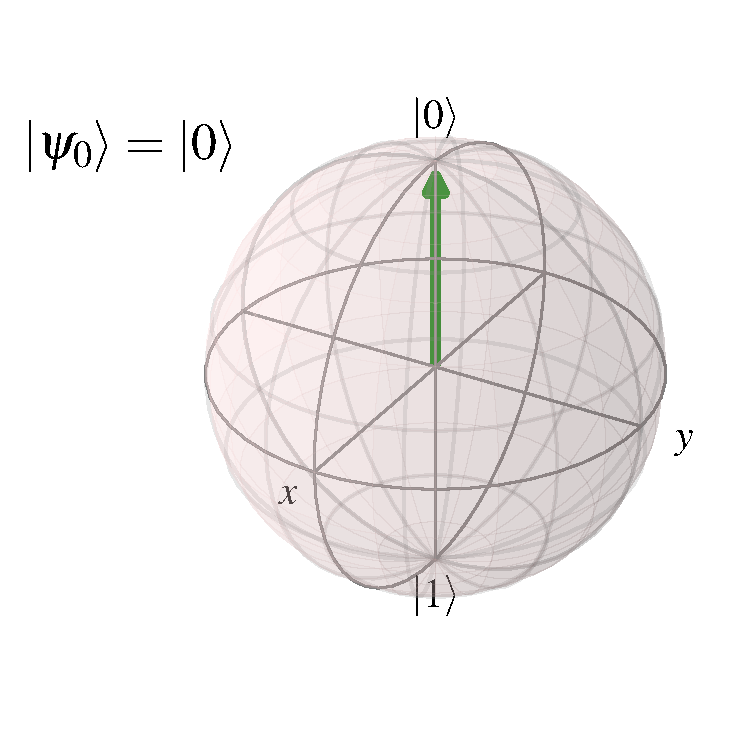
\includegraphics[width=0.28\textwidth]{experimental_study/figures/hahn_bloch_spheres/bloch_0.pdf}
        }
        \qquad
        \subfloat{
            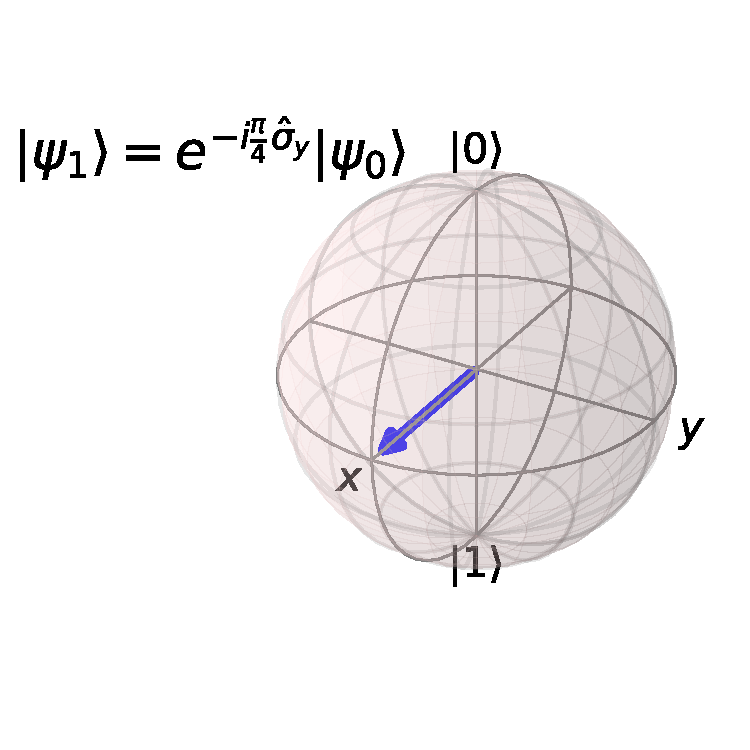
\includegraphics[width=0.28\textwidth]{experimental_study/figures/hahn_bloch_spheres/bloch_1.pdf}
        }
        \qquad
        \subfloat{
            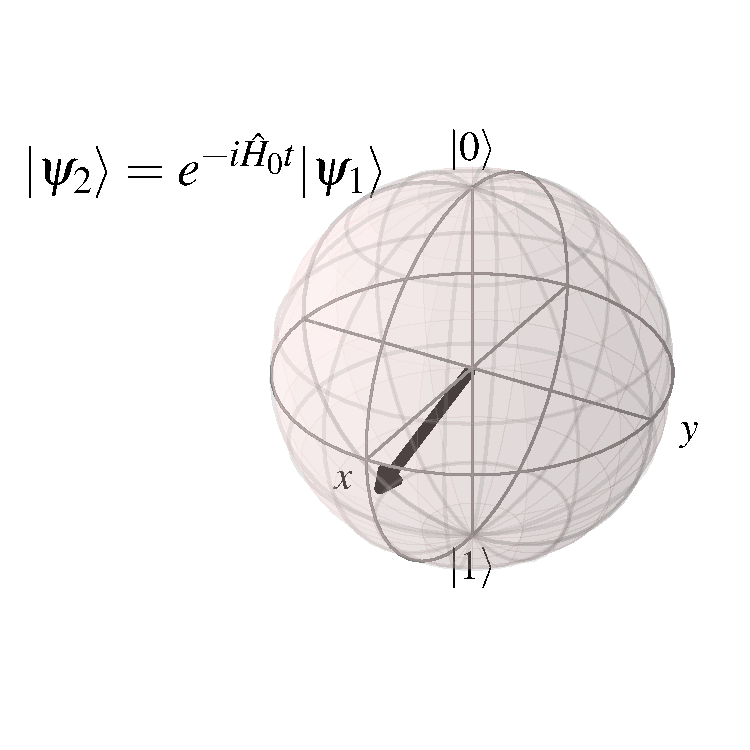
\includegraphics[width=0.28\textwidth]{experimental_study/figures/hahn_bloch_spheres/bloch_2.pdf}
        }
        \qquad
        \subfloat{
            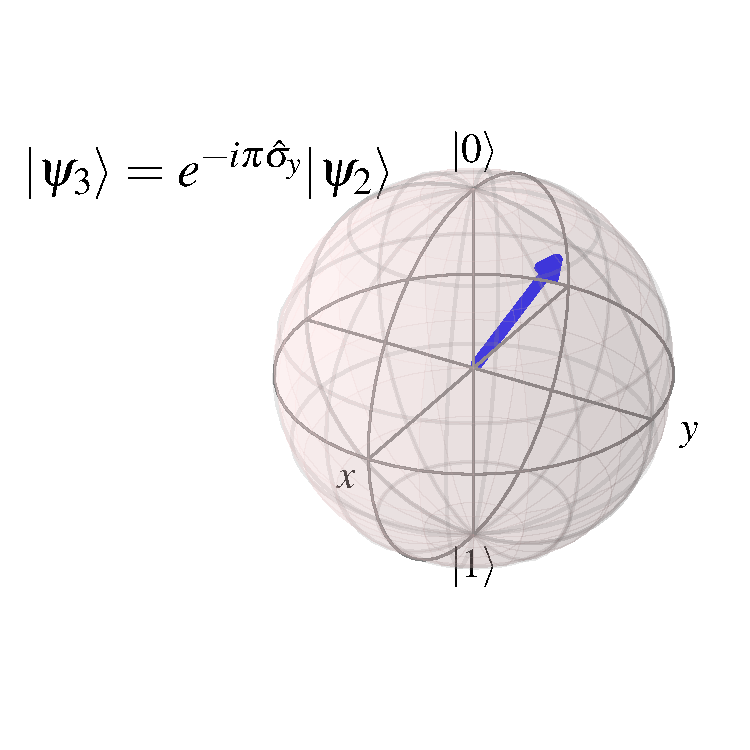
\includegraphics[width=0.28\textwidth]{experimental_study/figures/hahn_bloch_spheres/bloch_3.pdf}
        }
        \qquad
        \subfloat{
            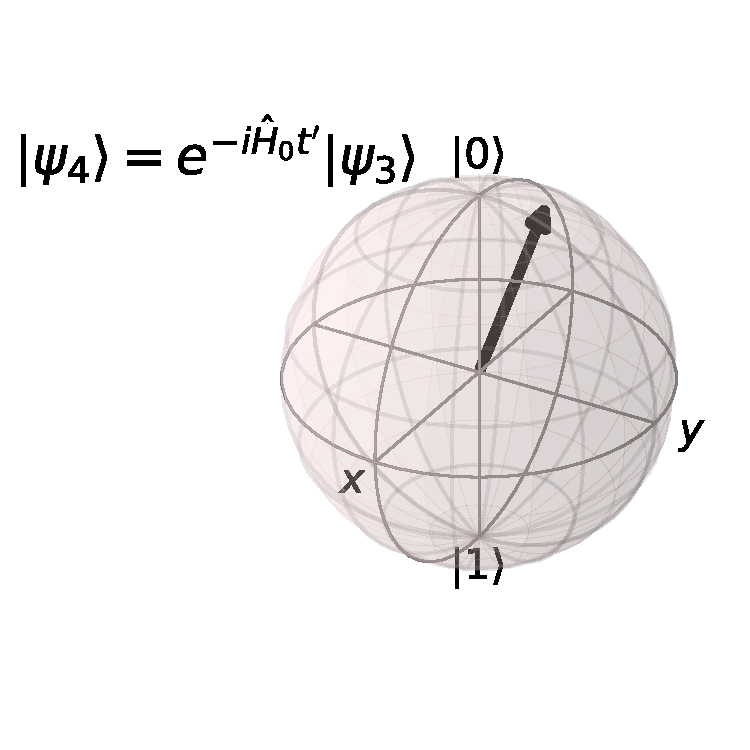
\includegraphics[width=0.28\textwidth]{experimental_study/figures/hahn_bloch_spheres/bloch_4.pdf}
        }
        \qquad
        \subfloat{
            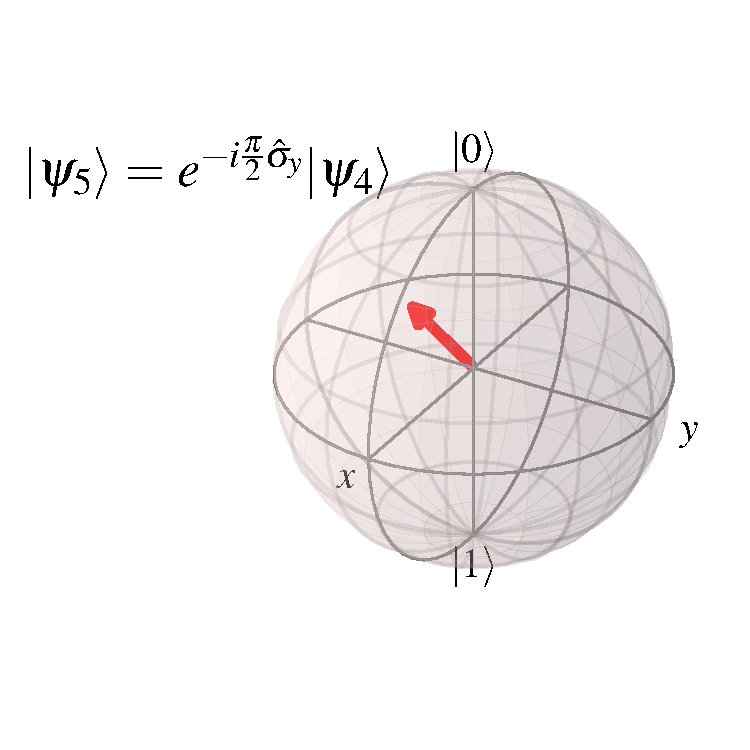
\includegraphics[width=0.28\textwidth]{experimental_study/figures/hahn_bloch_spheres/bloch_5.pdf}
        }
    \end{center}
    \caption[States of spin qubit at each stage of Hahn echo sequence]{
        States of spin qubit at each stage of Hahn echo sequence.
        
        The state of the \gls{nvc} spin is initialised by a green laser into state $\ket{\psi_0} = \ket{0}$. 
        We then apply a rotation about the $y$-axis (i.e. a \gls{mw} pulse), 
            yielding the state $\ket{\psi_1} = \ket{+}$. 
        The system is then allowed to evolve according to its own $\ho$ for $t$, $\ket{\psi_2} = e^{-i\ho t}\ket{+}$.
        We apply a second \gls{mw} pulse, this time for a $\pi$-rotation about the $y$-axis, 
        $\ket{\psi_3} = e^{-i\pi \s_y}e^{-i\ho t}\ket{+}$.
        Again the system evolves according to interactions with the environment, this time for $2t$.
        We apply a final \gls{mw} pulse to rotate about the $y$-axis again, 
            effectively either returning the spin to near the $\ket{0}$ axis, 
            or near the $\ket{1}$ axis. 
        Here $\ket{\psi}_5$ is roughly half way between $\ket{0}$ and $ket{+}$, 
        i.e. along the $z$-axis. 
        The spin is read out from $\ket{\psi}_5$ via the \gls{nvc}'s \glsentrylong{pl}. 
        Here $\ho = 0.25 \ \s_y$ was evolved for $t=0.5$ (arbitrary units), 
        and the final state overlap with the initial state, 
        i.e. the likelihood of measuring the spin in $\ket{0}$ is $\Pr(0 | \ho, t) = 0.865$. 
    }
    \label{fig:hahn_bloch_spheres}
\end{figure}
    
We have decided to characterise the hyperfine interactions of the \gls{nvc}; 
    these are evident most strongly at very short timescales \cite{childress2006coherent}. 
To isolate the effects of the hyperfine interactions, 
    we run Hahn echo experiments, which are known to emphasise weak interactions.
Hahn echo sequences attempt to decouple the spin's dynamics from the nuclear bath
    \cite{rowan1965electron, blok2014manipulating, childress2006coherent, charnock2001combined, gentile2020Operating}
    providing a helpful platform for studying residual contributions of terms in \cref{eqn:nv_terms}.
The \gls{nvc} qubit undergoes a series of evolutions -- either according to application of quantum logic gates
    or the natural evolution of the system interacting with its environmen  
We depict the stages of the experiment in \cref{fig:hahn_bloch_spheres}, 
    starting from the initialised $\ket{0}$
    through to its final state which is read out through \gls{pl},
    both of which as described in \cref{sec:nv_centres}.
\par 

In particular, the final state, $\ket{\psi}_5$, is read out, effectively by projection onto $\ket{0}$;
    we can interpret the \gls{pl} after evolution time $t$ as the \gls{likelihood} 
    that the \gls{nvc} is found in $\ket{0}$ after evolution of its \emph{true} Hamiltonian, $\ho$. 
That is, we assign this projection as the quantity $\Pr(0 | \ho, t)$ (the \gls{likelihood}), 
    and it can be used within likelihood estimation in order to refine a candidate model $\hj$, 
    effectively\footnotemark \ by changing the structure of 
    $\hj$ until $\Pr(0 | \ho, t) \approx \Pr(0 | \hj, t) \forall t$. 

\footnotetext{
    Of course this is a gross simplification of \gls{qhl} which is described fully in \cref{sec:qhl}
}
\par 

By varying the evolution time of the Hahn-echo sequence, we can map the likelihood 
    against time, which we can view as capturing the dynamics of the \gls{nvc} spin \cref{fig:exp_raw_data}.
We vary time up to $\sim 4 \mu s$ in the short-time-range; 
    we will consider longer time ranges in simulation in \cref{chapter:many_qubits}. 

\begin{figure}
    \begin{center}
        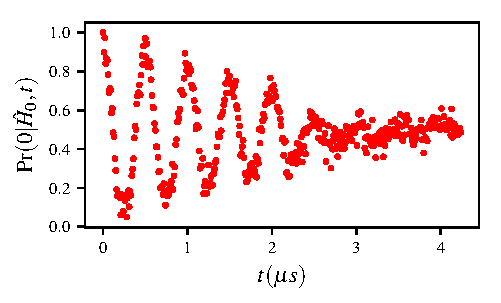
\includegraphics{experimental_study/figures/raw_data.pdf}
    \end{center}
    \caption[Raw data for the \glsentrylong{nvc}'s dynamics.]{
        Raw data for the \glsentrylong{nvc}'s dynamics.
        The $y$-axis shows the \glsentrylong{pl} of the \gls{nvc}, 
        equivalently the likelihood $\Pr(0 | \ho, t)$. 
    }
\end{figure}


\section{\glsentrylong{es}}
Finally, then, we are in a position to marry the concepts of 

\begin{figure}
    \label{fig:exp_qmla_analysis}
    \includegraphics[width=0.95\textwidth]{experimental_study/figures/experimental_qmla_analysis.pdf}
    \caption[\gls{qmla} applied to experimental system.]{
        \textbf{a}, 
        The carbon lattice providing the outer environment for the NV centre, along with the
        time evolution of the electron spin state (represented on a Bloch sphere) during the pulses for the Hahn-echo sequences. The final $\pi/2$ pulse is omitted.  
        \textbf{b}, 
        Simulation of 500 independent \gls{qmla} instances, where $\ho$ is chosen randomly. 
        The win rate is reported against the difference $(N_{p}-N^{\prime}_p)$ between the 
        number of parameters in the \gls{qmla}-selected ($\hp$) and true models, respectively. 
        The \emph{under-parameterised} \emph{ (over-parameterised)} class refers to models with less (more) 
        parameters than $\ho$. 
        \emph{Correct} indicates that exactly $\ho$ was found. 
        The \emph{mis-parameterised} class groups models with the same parametrisation cardinality as $\ho$, but different Hamiltonian terms. 
        \textbf{Inset}, Histogram of occurrences of $R^2$ values for each retrieved $\hp$ 
        against a sampling of datapoints from $\ho$, with median $R^2=0.84$ (red dotted line). 
        \textbf{c}, 
        Win rates of top four models (see main text), for 100 \gls{qmla} instances, 
        against both simulated and experimental data. 
        Simulations use $\ho = \hat{S}xyzAz$.
        \textbf{d}, 
        Total volume spanned by the parameters' prior across epochs, for the models in \textbf{c}. 
        Shaded areas indicate $66\%$ credible regions. 
        \textbf{e}, 
        Simulated likelihoods reproduced by the model with the highest win rate ($\hat{S}_{x,y,z}\hat{A}_{z}$, turquoise), compared with corresponding NV-centre system experimental data (red-dots, extracted from the observed \gls{pl} {of the first microseconds in Hahn-echo decay}). 
        Error bars smaller than the dots (see Methods).
        \textbf{f}, 
        A single QMLA instance against experimental data in \textbf{e}, depicted as a \gls{cdag}, see Fig.~\ref{fig:Fig1}c.
        The thin end of each edge points to the favoured model; 
        the colour of the edges maps $\log_{10}\mathcal{B}$ as in the bar legend at the bottom. 
        Layer champions \huc are in light brown, whereas the global champion $\hp$  is in orange.    
    }
\end{figure}